\section{Class Diagram}

The class diagram showed in figure \ref{fig:diagram} is made to show the relation between the GirafRecord class and some of the other classes used in the Giraf system.
Besides the GirafRecord class, all the other included classes are subclasses of the GirafRecord class. This means that the subclasses inherit all the functions and attributes from the GirafRecord class.
The subclasses of the GirafRecord class can override some function and attributes of the main class, and other functions and attributes has to be overridden by the subclasses, these functions and attributes are the ones which is shown in all included classes in figure \ref{fig:diagram}.
An example of this, is the attribute 'RETURN\_PRIMARYKEY' and the function 'getPrimaryKey()'.
  
\begin{figure}[h]
\centering
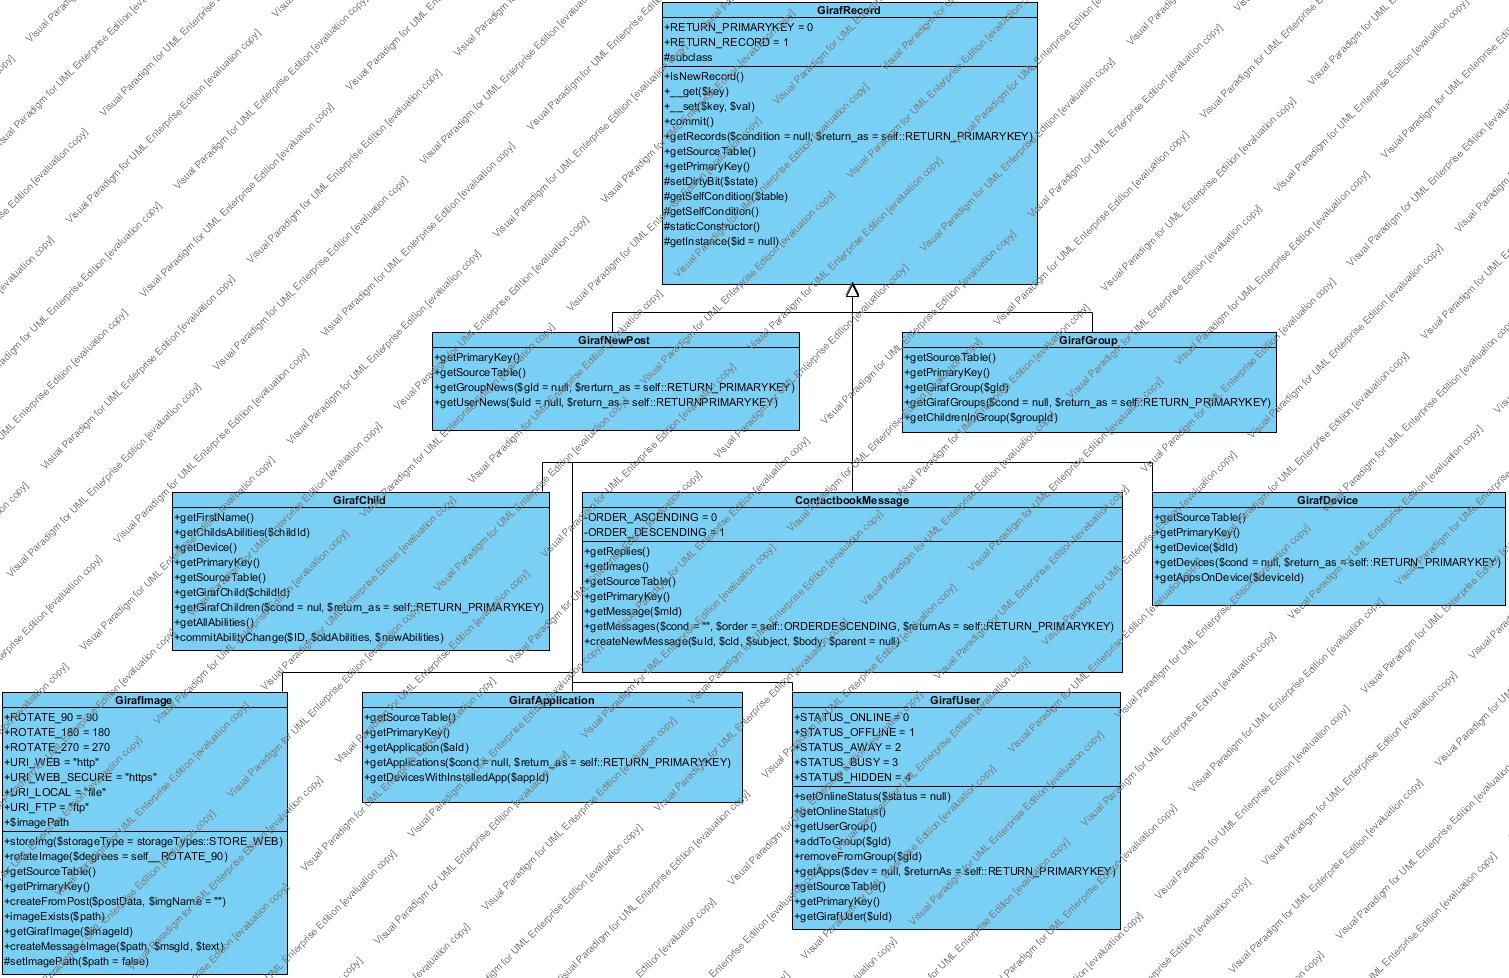
\includegraphics[width=250px]{img/classdiagram_Project.jpg}
\caption{The figure shows the class diagram of the GirafRecord class, and its subclasses}
\label{fig:diagram}
\end{figure}

\section{Component architecture}

The architecture of the administrations part of the Giraf system is designed as a client-server architecture. Which means that the user uses the client to communicate with the server, at which the database lies. Within the client and the server lies three components. These components i called; view, controller and database. These three components communicates with each other in the way that the the view communicates with the database through the controller. Which means that the controller is the link between the two other components. Even though the architecture of the system is client-server, it is designed such that the client does not contain any components, and therefore the server contain all the three components, the reason is that the system is 100\% internet based, which means that all the components of the system lies at the servers site. The componentarchitecture can be seen in figure \ref{fig:architecture}

\begin{figure}[!h]
\centering
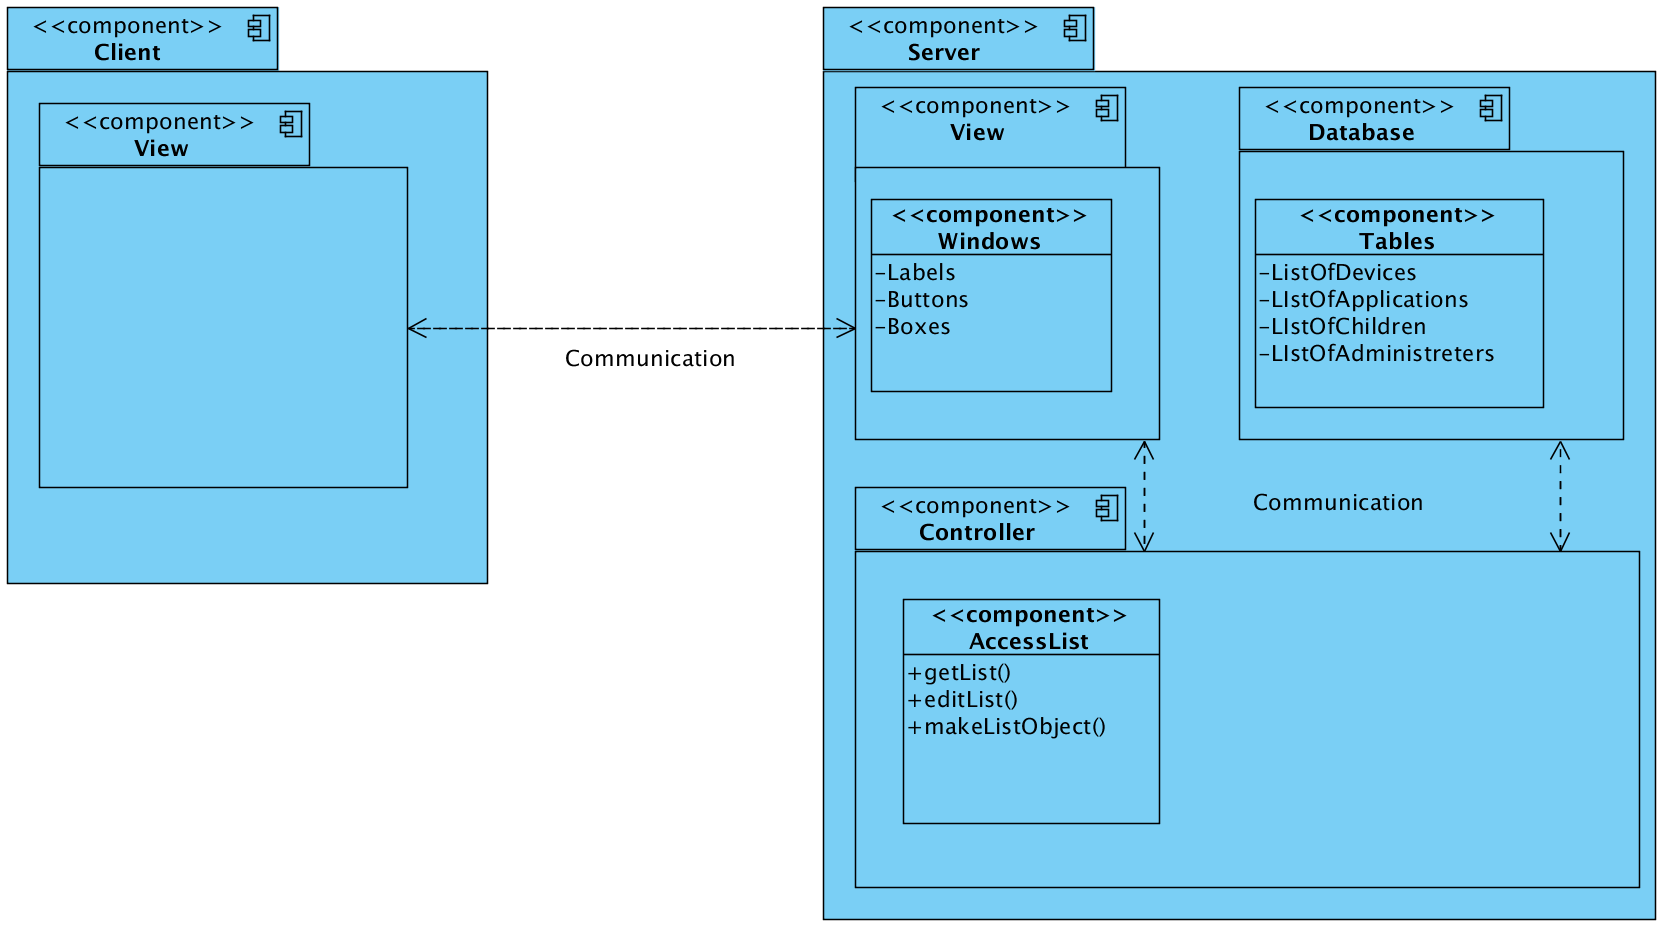
\includegraphics[width=300px]{img/ComponentArketektur.png}
\caption{The figure shows the component architecture of the administrations system}
\label{fig:architecture}
\end{figure}

The three components contains other components, which contains some attributes. These attributes defines what function the overall component has, for example contains the view component a windows component, which contains some attributes called 'labels', 'buttons' and 'boxes'.The attributes shows that the windows component can indicate labels, buttons and boxes.
The controller contains a component with some attributes which indicates that the accesList can, get a list from the database, edit a list from the database and make an object of a list.
The database component contains a component called lists, this component has an attribute called lists, this attribute indicates that the database contains lists. Among these lists is a list of devices, a list of children, a list of applications and a list of administrators.